\documentclass[11pt]{beamer}
\usetheme{simple}
\setbeamertemplate{footline}{} 
\usepackage{tikz, pgfplots,amsmath, amssymb, amsthm}   
\usepgfplotslibrary{groupplots}

\usepackage{sansmathaccent}
\pdfmapfile{+sansmathaccent.map}


%\pgfplotsset{ every non boxed y axis/.append style={y axis line style=-}}
\setbeamertemplate{navigation symbols}{}
\begin{document}
\begin{frame}




\only<1>{
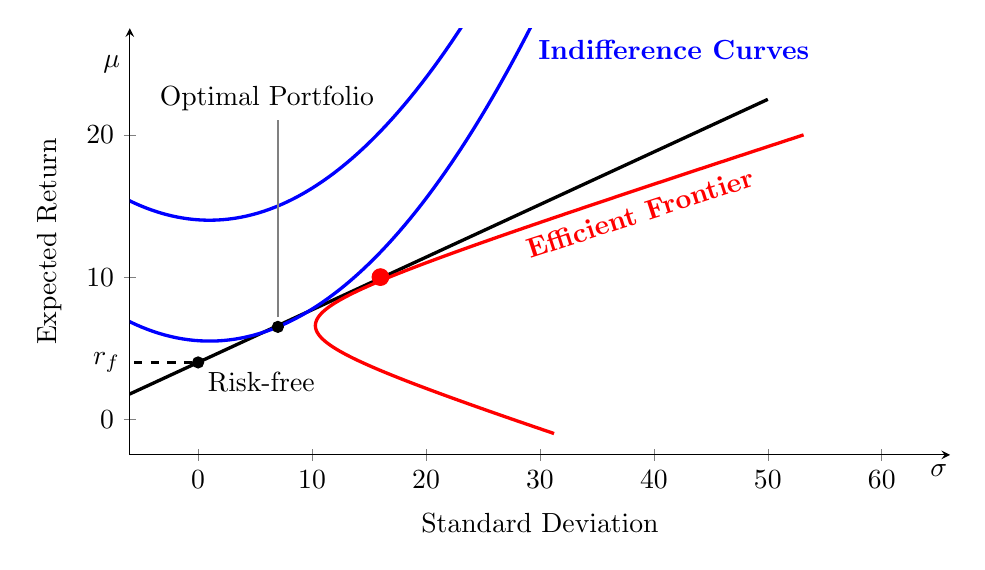
\begin{tikzpicture}
\begin{axis}[
  height=7cm, width=12cm,
  axis x line=bottom, axis y line=left,
  xlabel = Standard Deviation, ylabel = Expected Return,
  ymin=0, ymax=25, xmin=0, xmax=60,
  extra x ticks={65}, extra x tick labels={$\sigma$},
  extra x tick style={major tick length=0mm, grid=none},
  extra y ticks={4,25}, extra y tick labels={$r_f$ , $\mu$},
  extra y tick style={major tick length=0mm,  grid=none},
  enlargelimits=true,
  scatter/classes={
    a={mark=o,draw=black, mark size = 3pt},
    b={mark=*, mark size = 3pt,draw=red, fill = red}
    }
]

\addplot[black, very thick, domain=-10:50, samples=100, variable=\x](
  ({x}, {4 + 0.37 * x});
\addplot[scatter,only marks, scatter src=explicit symbolic]
  coordinates {
    (7, 6.5)     [c]
    (0, 4)      [c]
    (16, 10)     [b]
  };
%node at (axis cs:12, 5) [anchor=south west] {A};
%node at (axis cs:7,6.5) [anchor=north west] {Optimal Portfolio};
\node at (axis cs:0,4) [anchor=north west] {Risk-free };
%\node[color=red] at (axis cs:16,10) [anchor=south east] {Market Portfolio};
\addplot[blue, very thick,  domain=-7:10, samples=200, variable=\t](
  {11 * t + (1-t) * 5-10},{(t-1)^2+5.5 } %{(t^2 * 20^2 + (1-t)^2 * 12)},
   );
 \addplot[blue, very thick,  domain=-7:10, samples=200, variable=\t](
  {11 * t + (1-t) * 5-10},{(t-1)^2+14 } %{(t^2 * 20^2 + (1-t)^2 * 12)},
   )  ;
 \node[color=blue] at (axis cs:29, 26) [anchor=west] {\textbf{Indifference Curves}};
\node[rotate=18, color=red] at (axis cs:50, 16) [anchor=south east] {\textbf{Efficient Frontier}};
\node[pin={[pin edge={thick}, text width=3cm, pin distance=2.5cm]90:{{\centering Optimal Portfolio}}}] at (axis cs:7, 6.5) {};
\draw[dashed, thick] (axis cs:-10,4) -- (axis cs:0,4);
% \draw[dashed, color=red,thick] (axis cs:-10,10) -- (axis cs:16, 10);
\addplot[red, very thick,  domain=-1:2.5, samples=200, variable=\t](
  {(20^2*t^2 + 12^2*(1-t)^2)^(0.5) }, %{(t^2 * 20^2 + (1-t)^2 * 12)},
  {11 * t + (1-t) * 5} );
\end{axis}   
\end{tikzpicture}}





\end{frame}
\end{document}